\chapter{Correlations}
\begin{figure}[htbp]
    \centering
     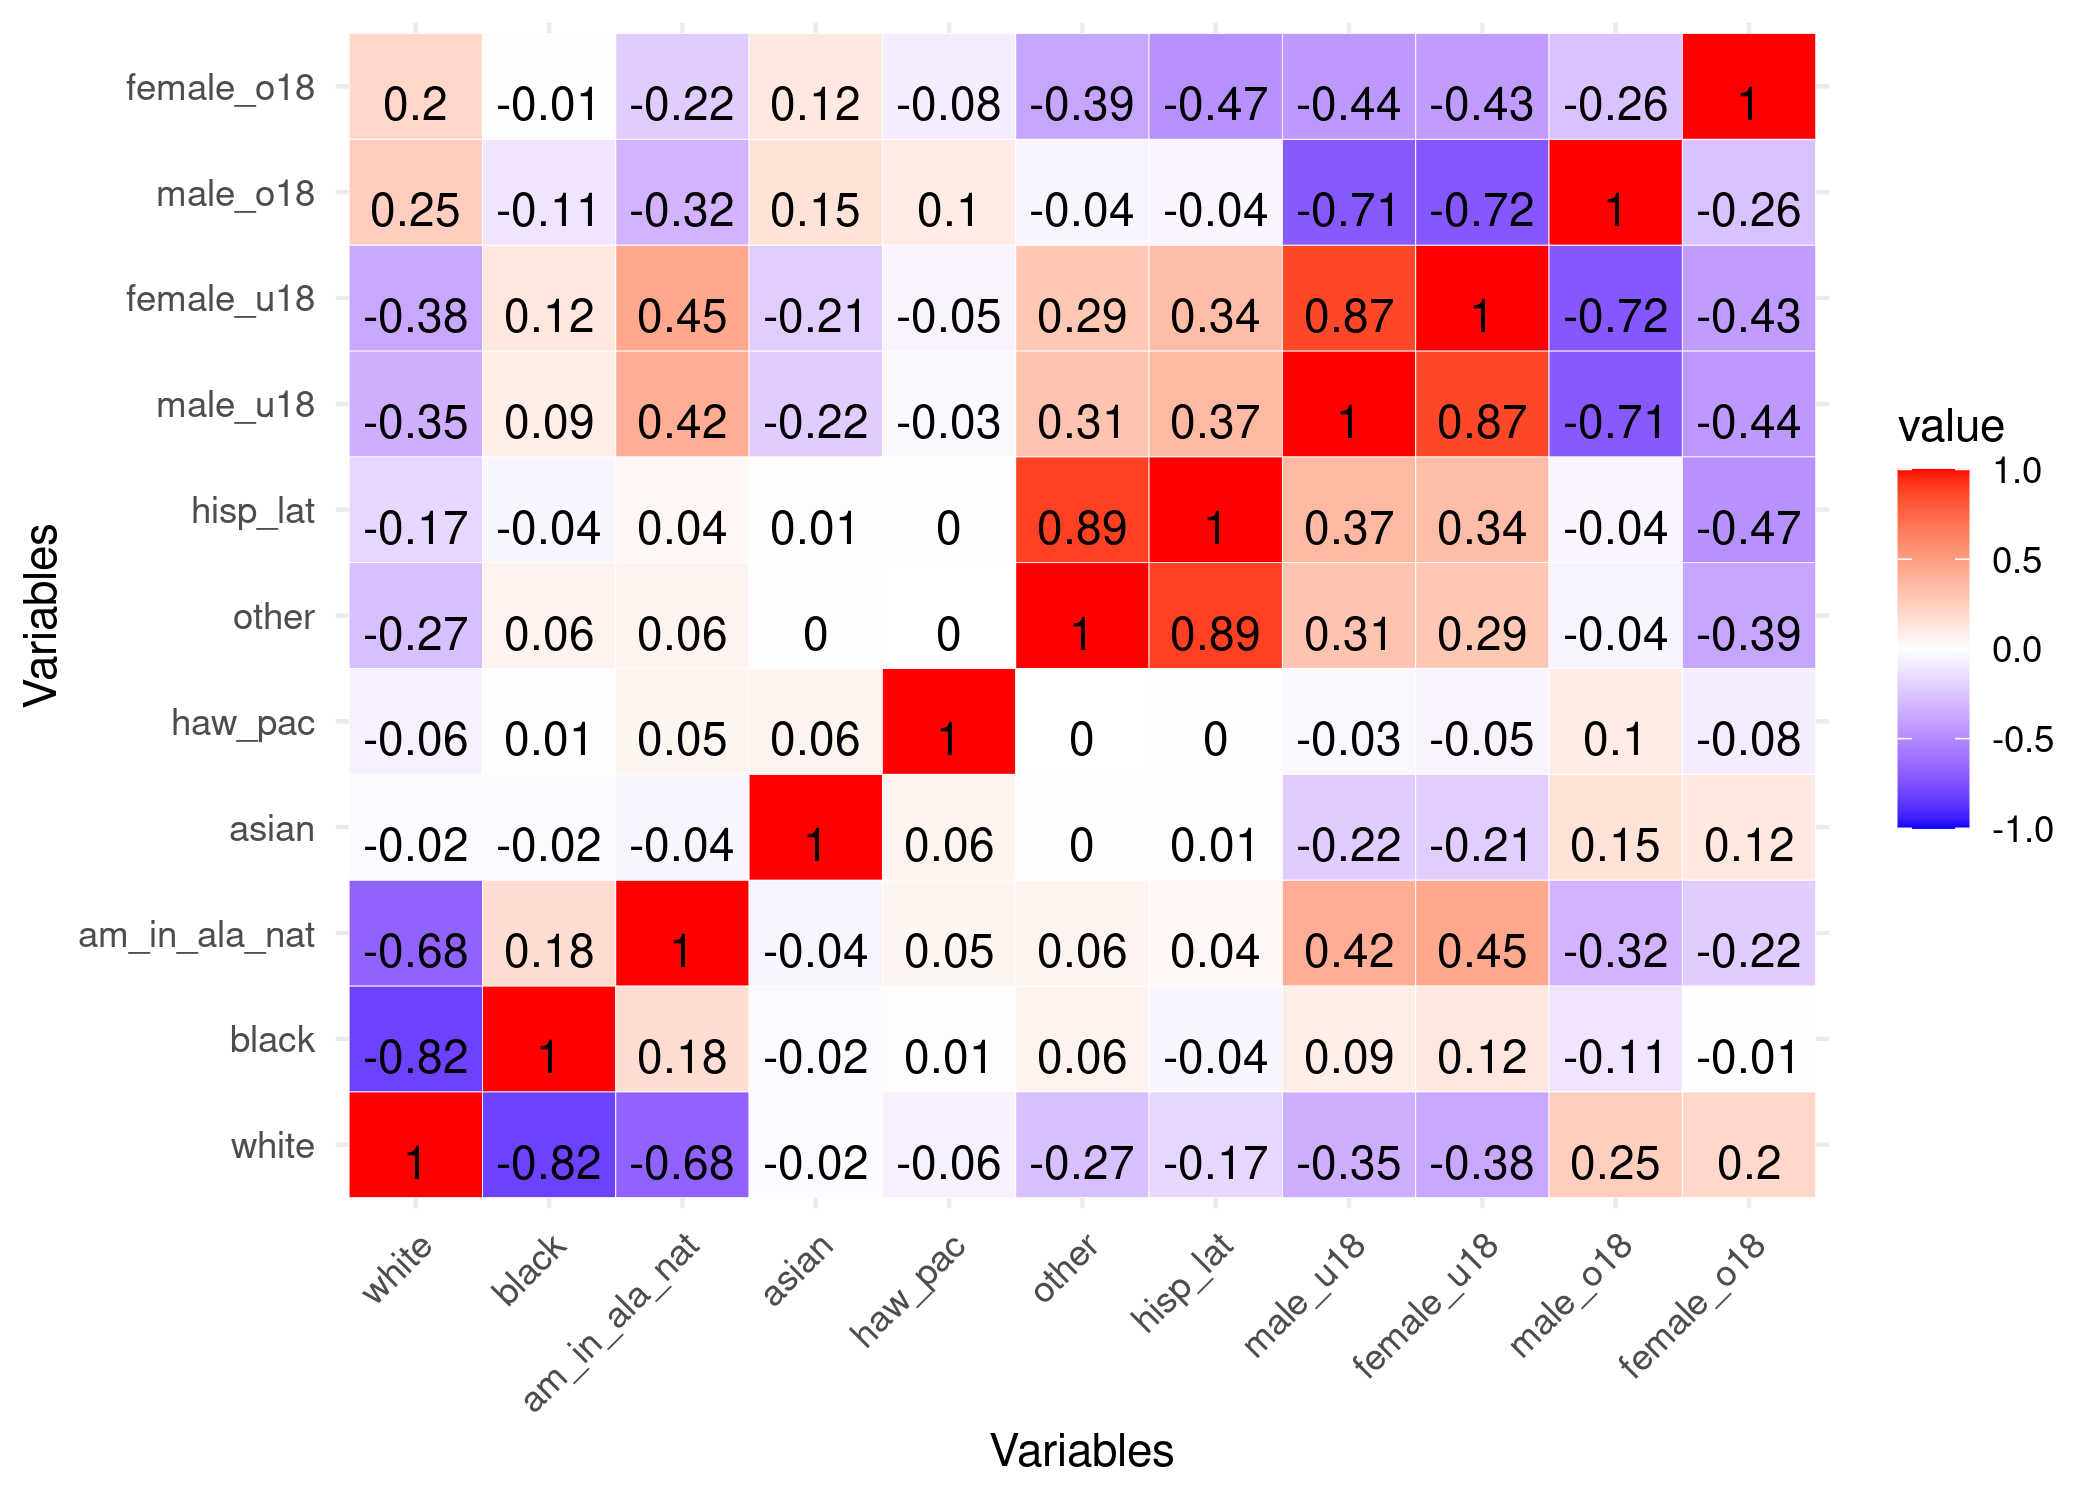
\includegraphics[width=1\textwidth, height=12cm]{plots/correlations/dem_prob_corr.png}
     \caption{Demographics Correlation Plot}
 \end{figure}

 \begin{figure}[htbp]
    \centering
     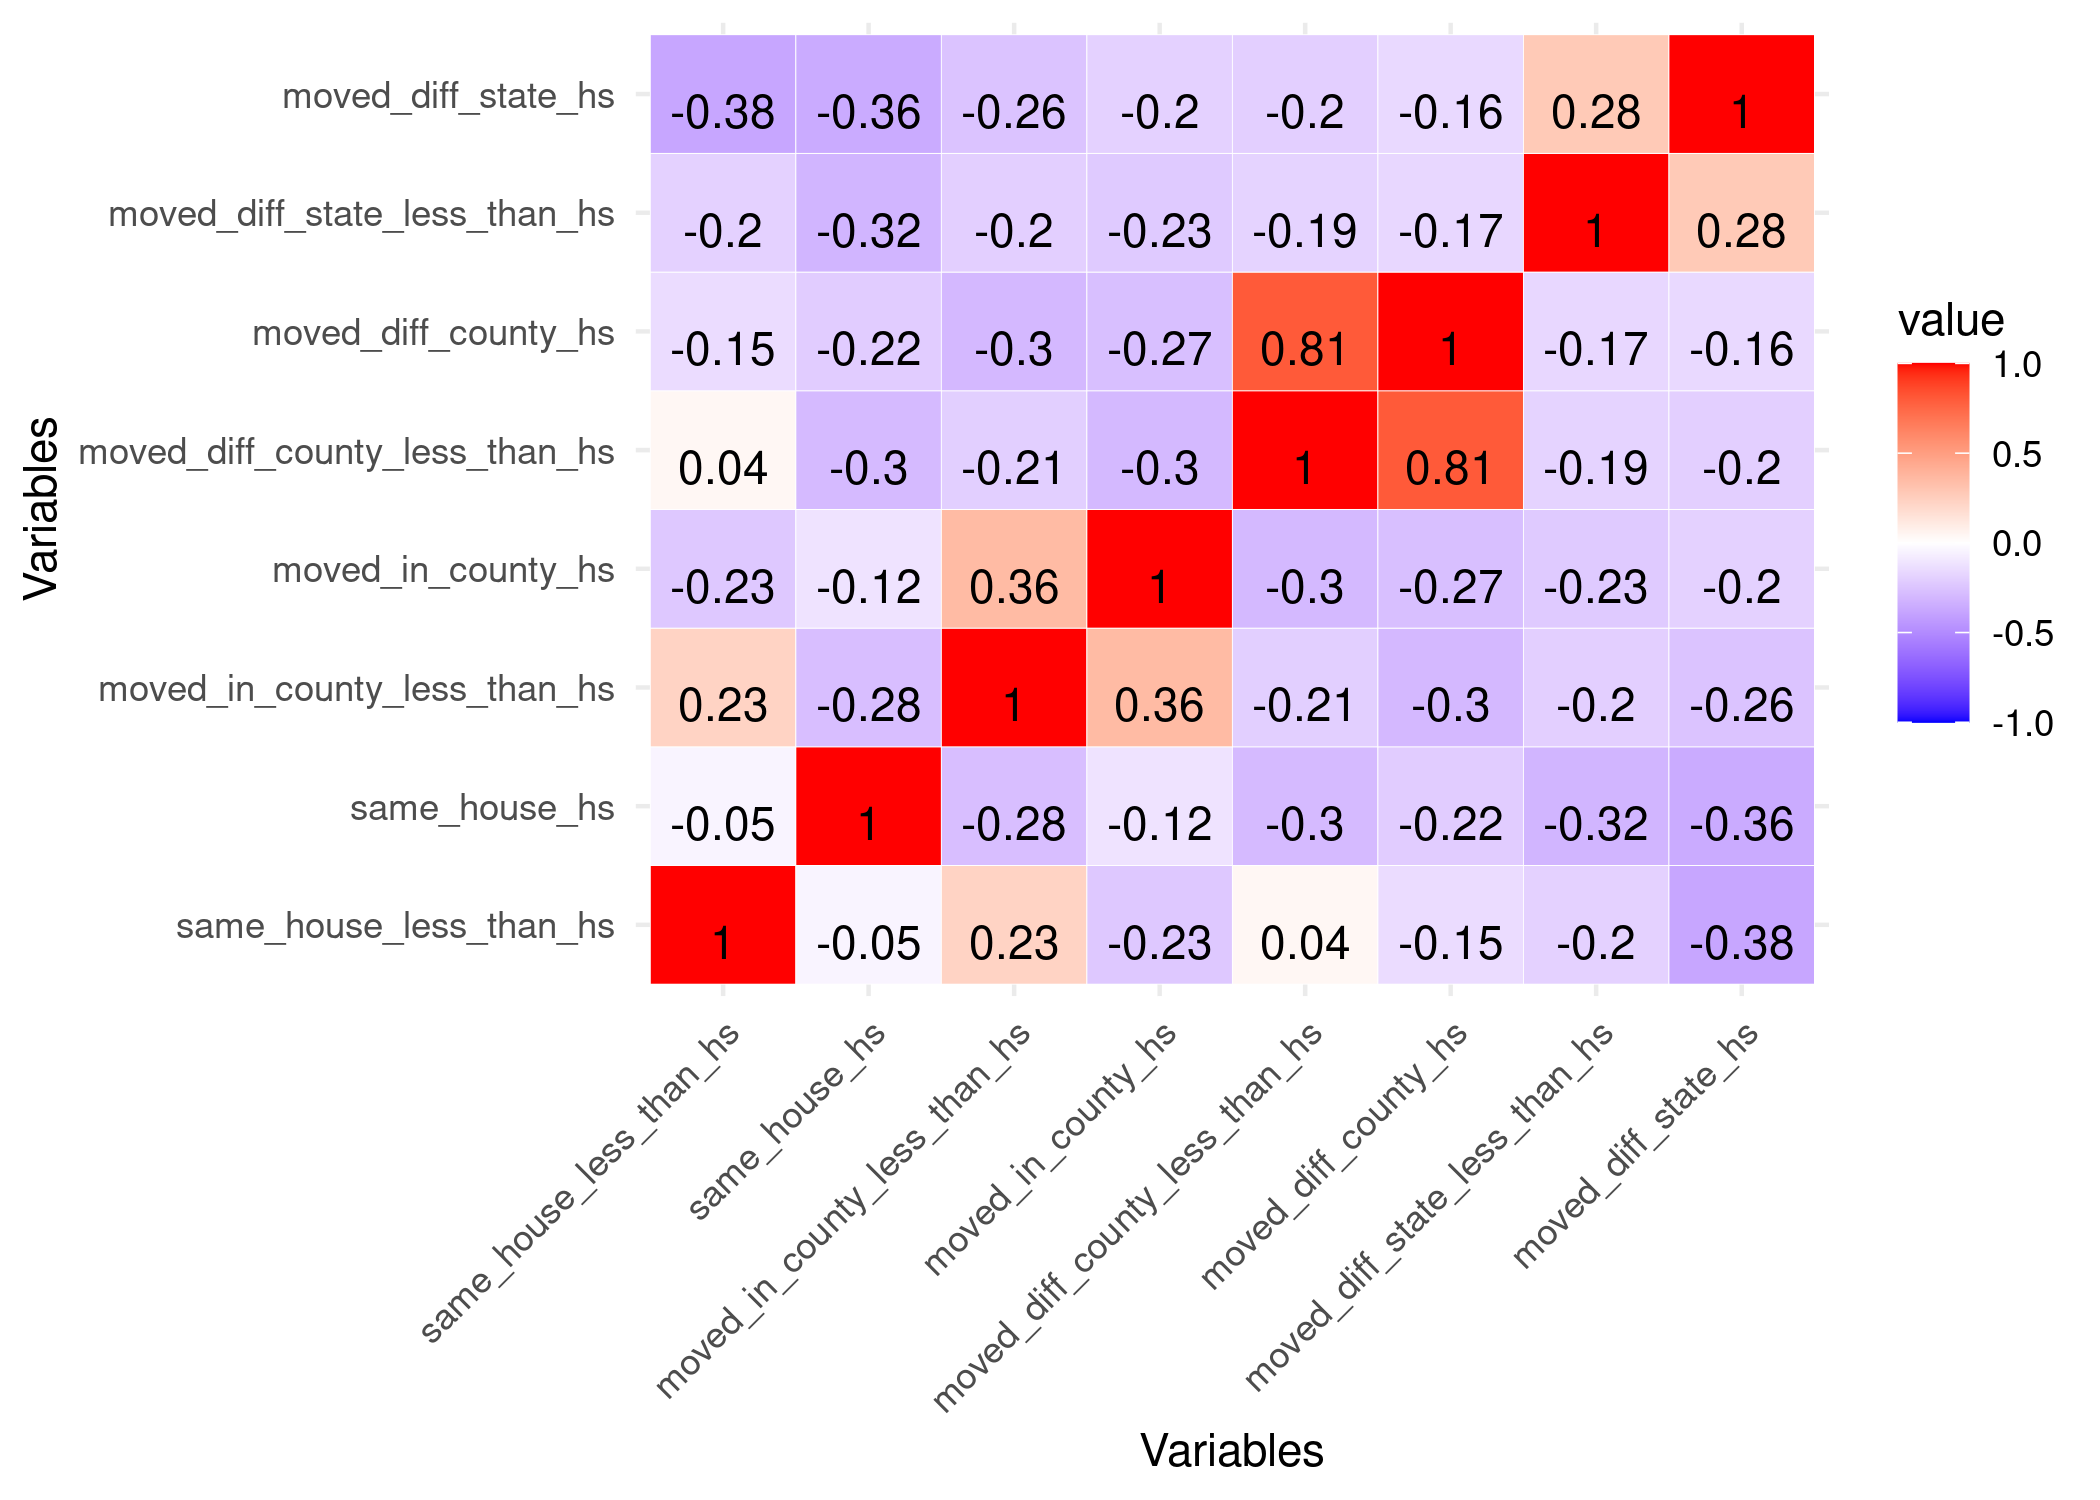
\includegraphics[width=1\textwidth, height=12cm]{plots/correlations/RME_prob_corr.png}
     \caption{RME Correlation Plot}
 \end{figure}

 \begin{figure}[htbp]
    \centering
     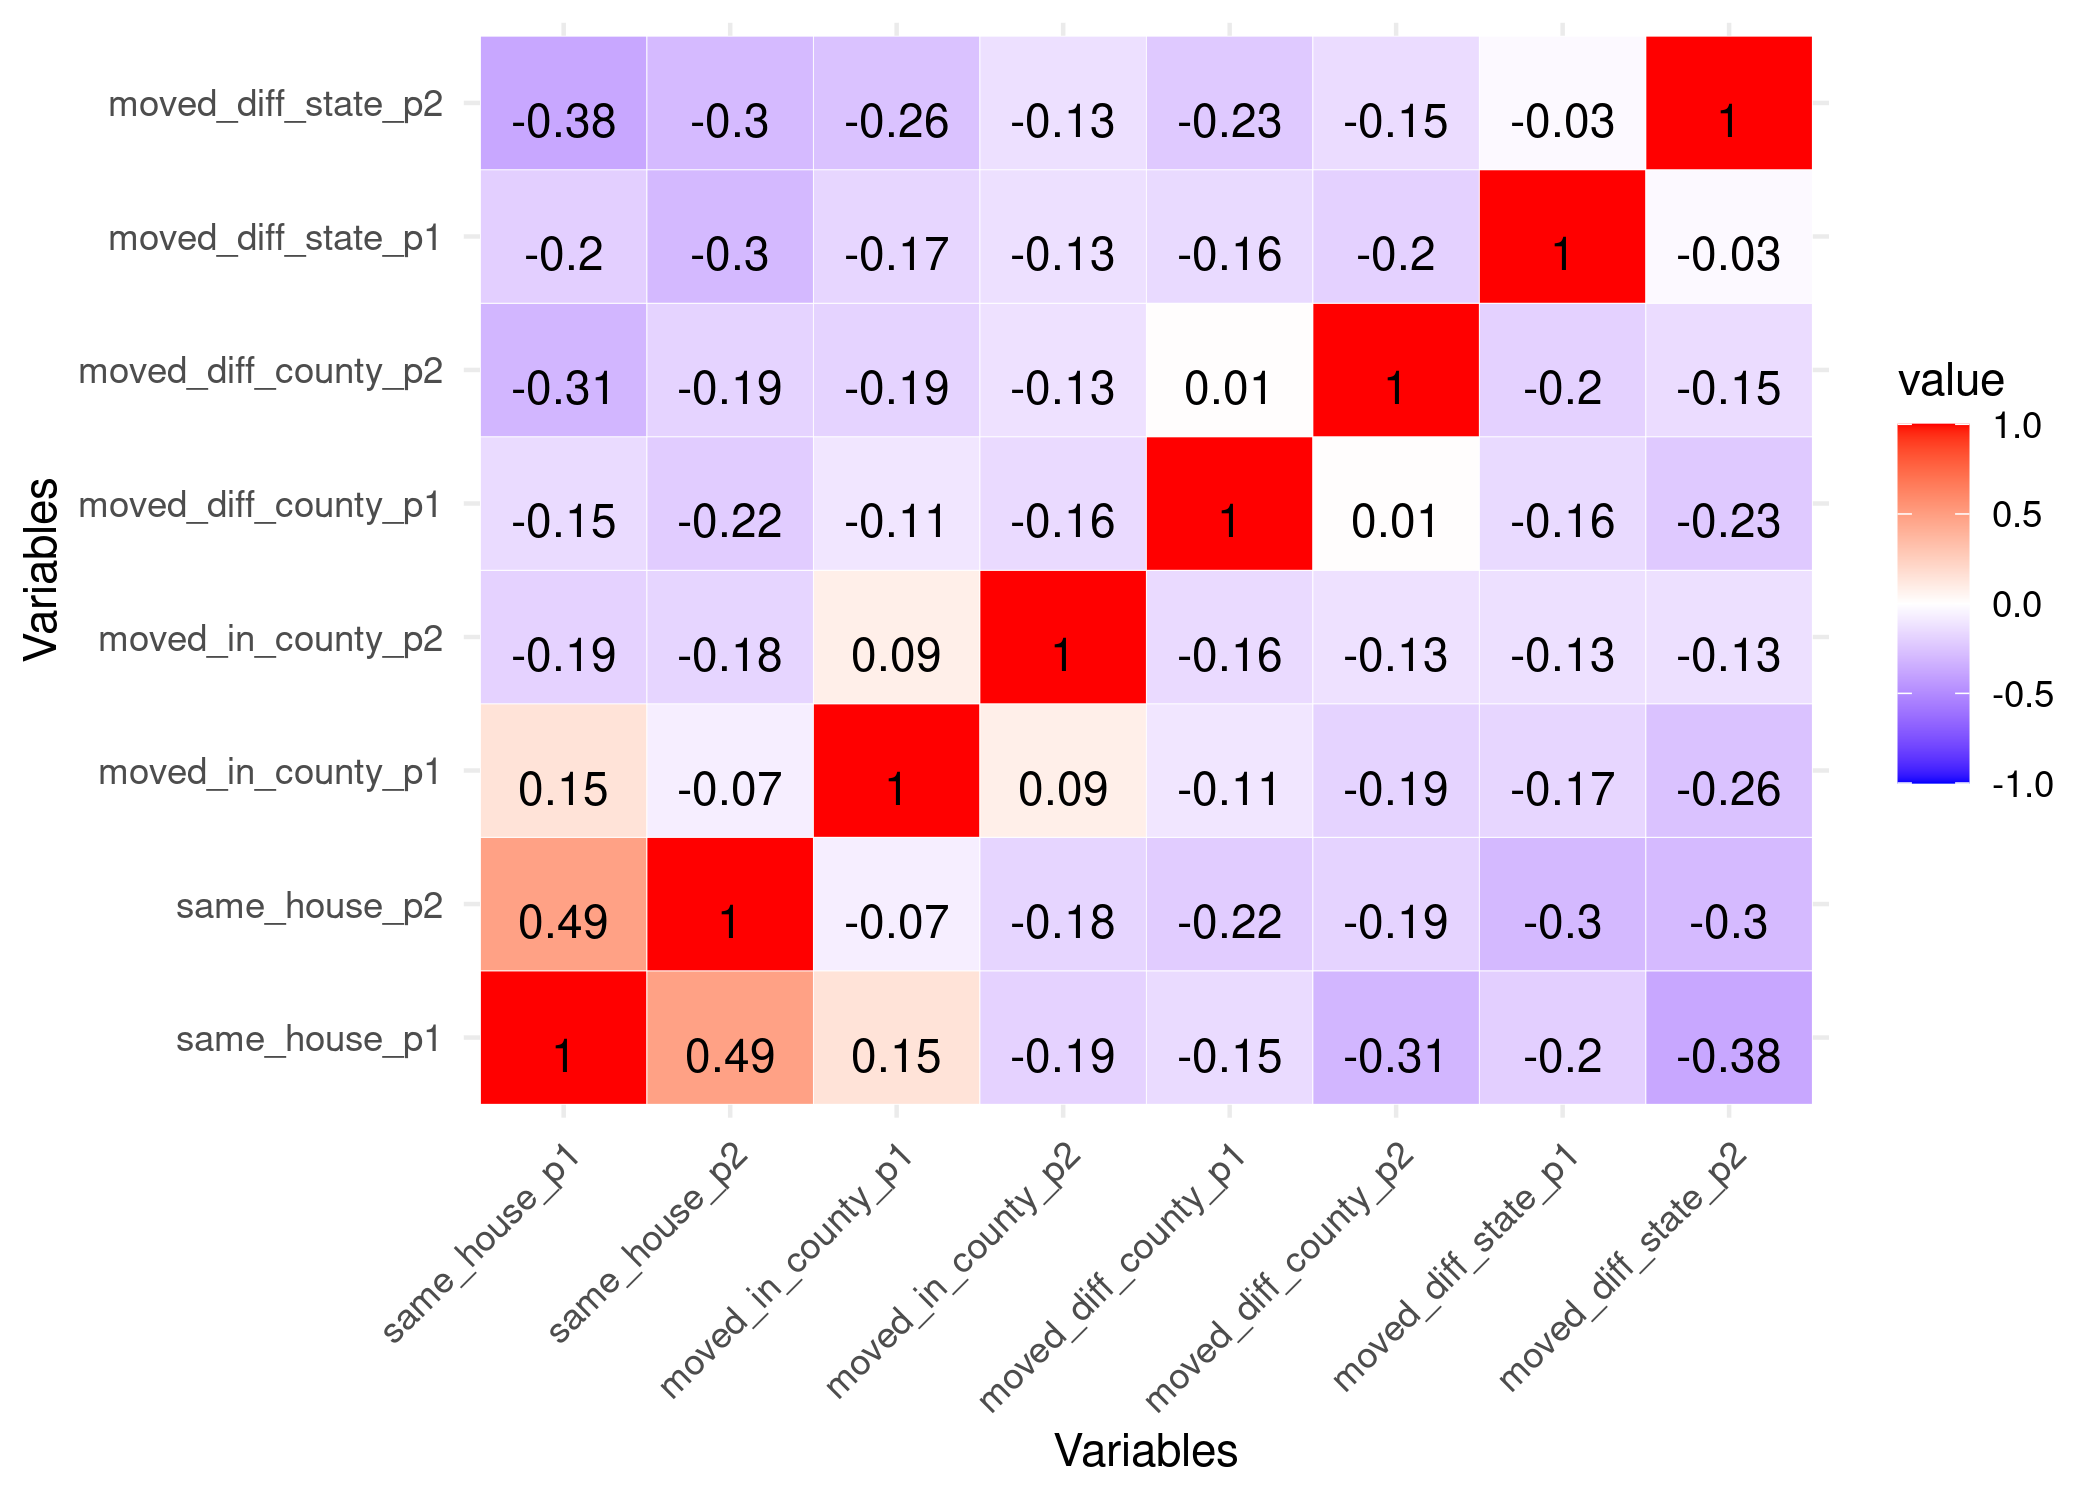
\includegraphics[width=1\textwidth, height=12cm]{plots/correlations/RMP_prob_corr.png}
     \caption{RME Correlation Plot}
 \end{figure}

 \begin{figure}[htbp]
    \centering
     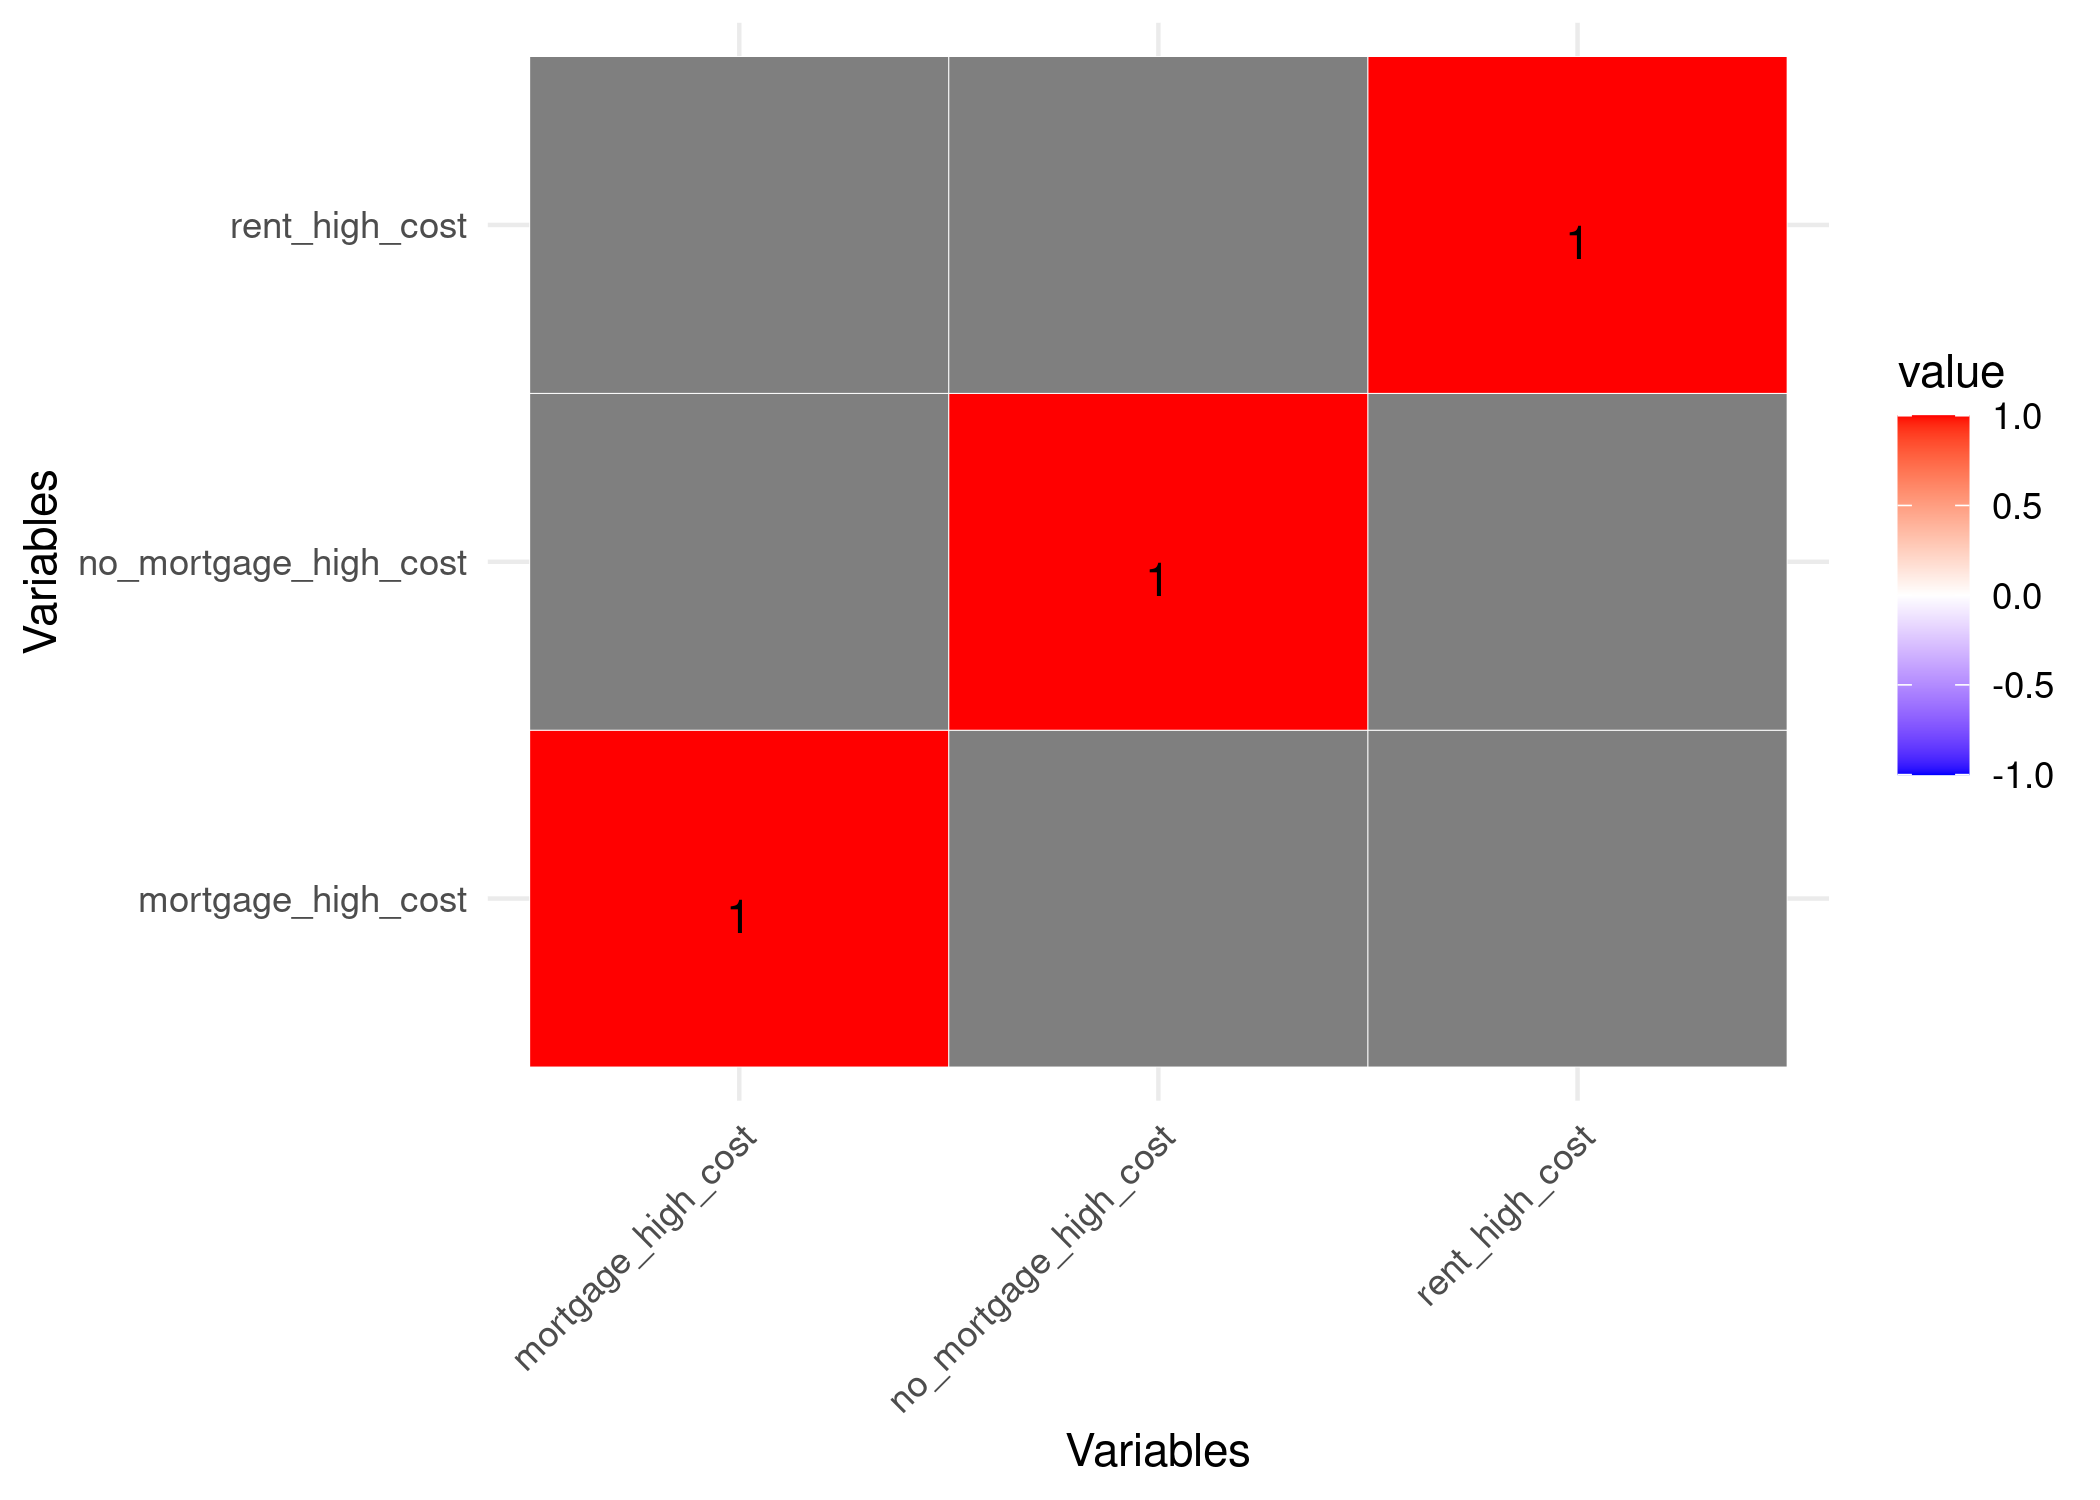
\includegraphics[width=1\textwidth, height=12cm]{plots/correlations/cost_prob_corr.png}
     \caption{Housing Costs Correlation Plot}
 \end{figure}

 \begin{figure}[htbp]
    \centering
     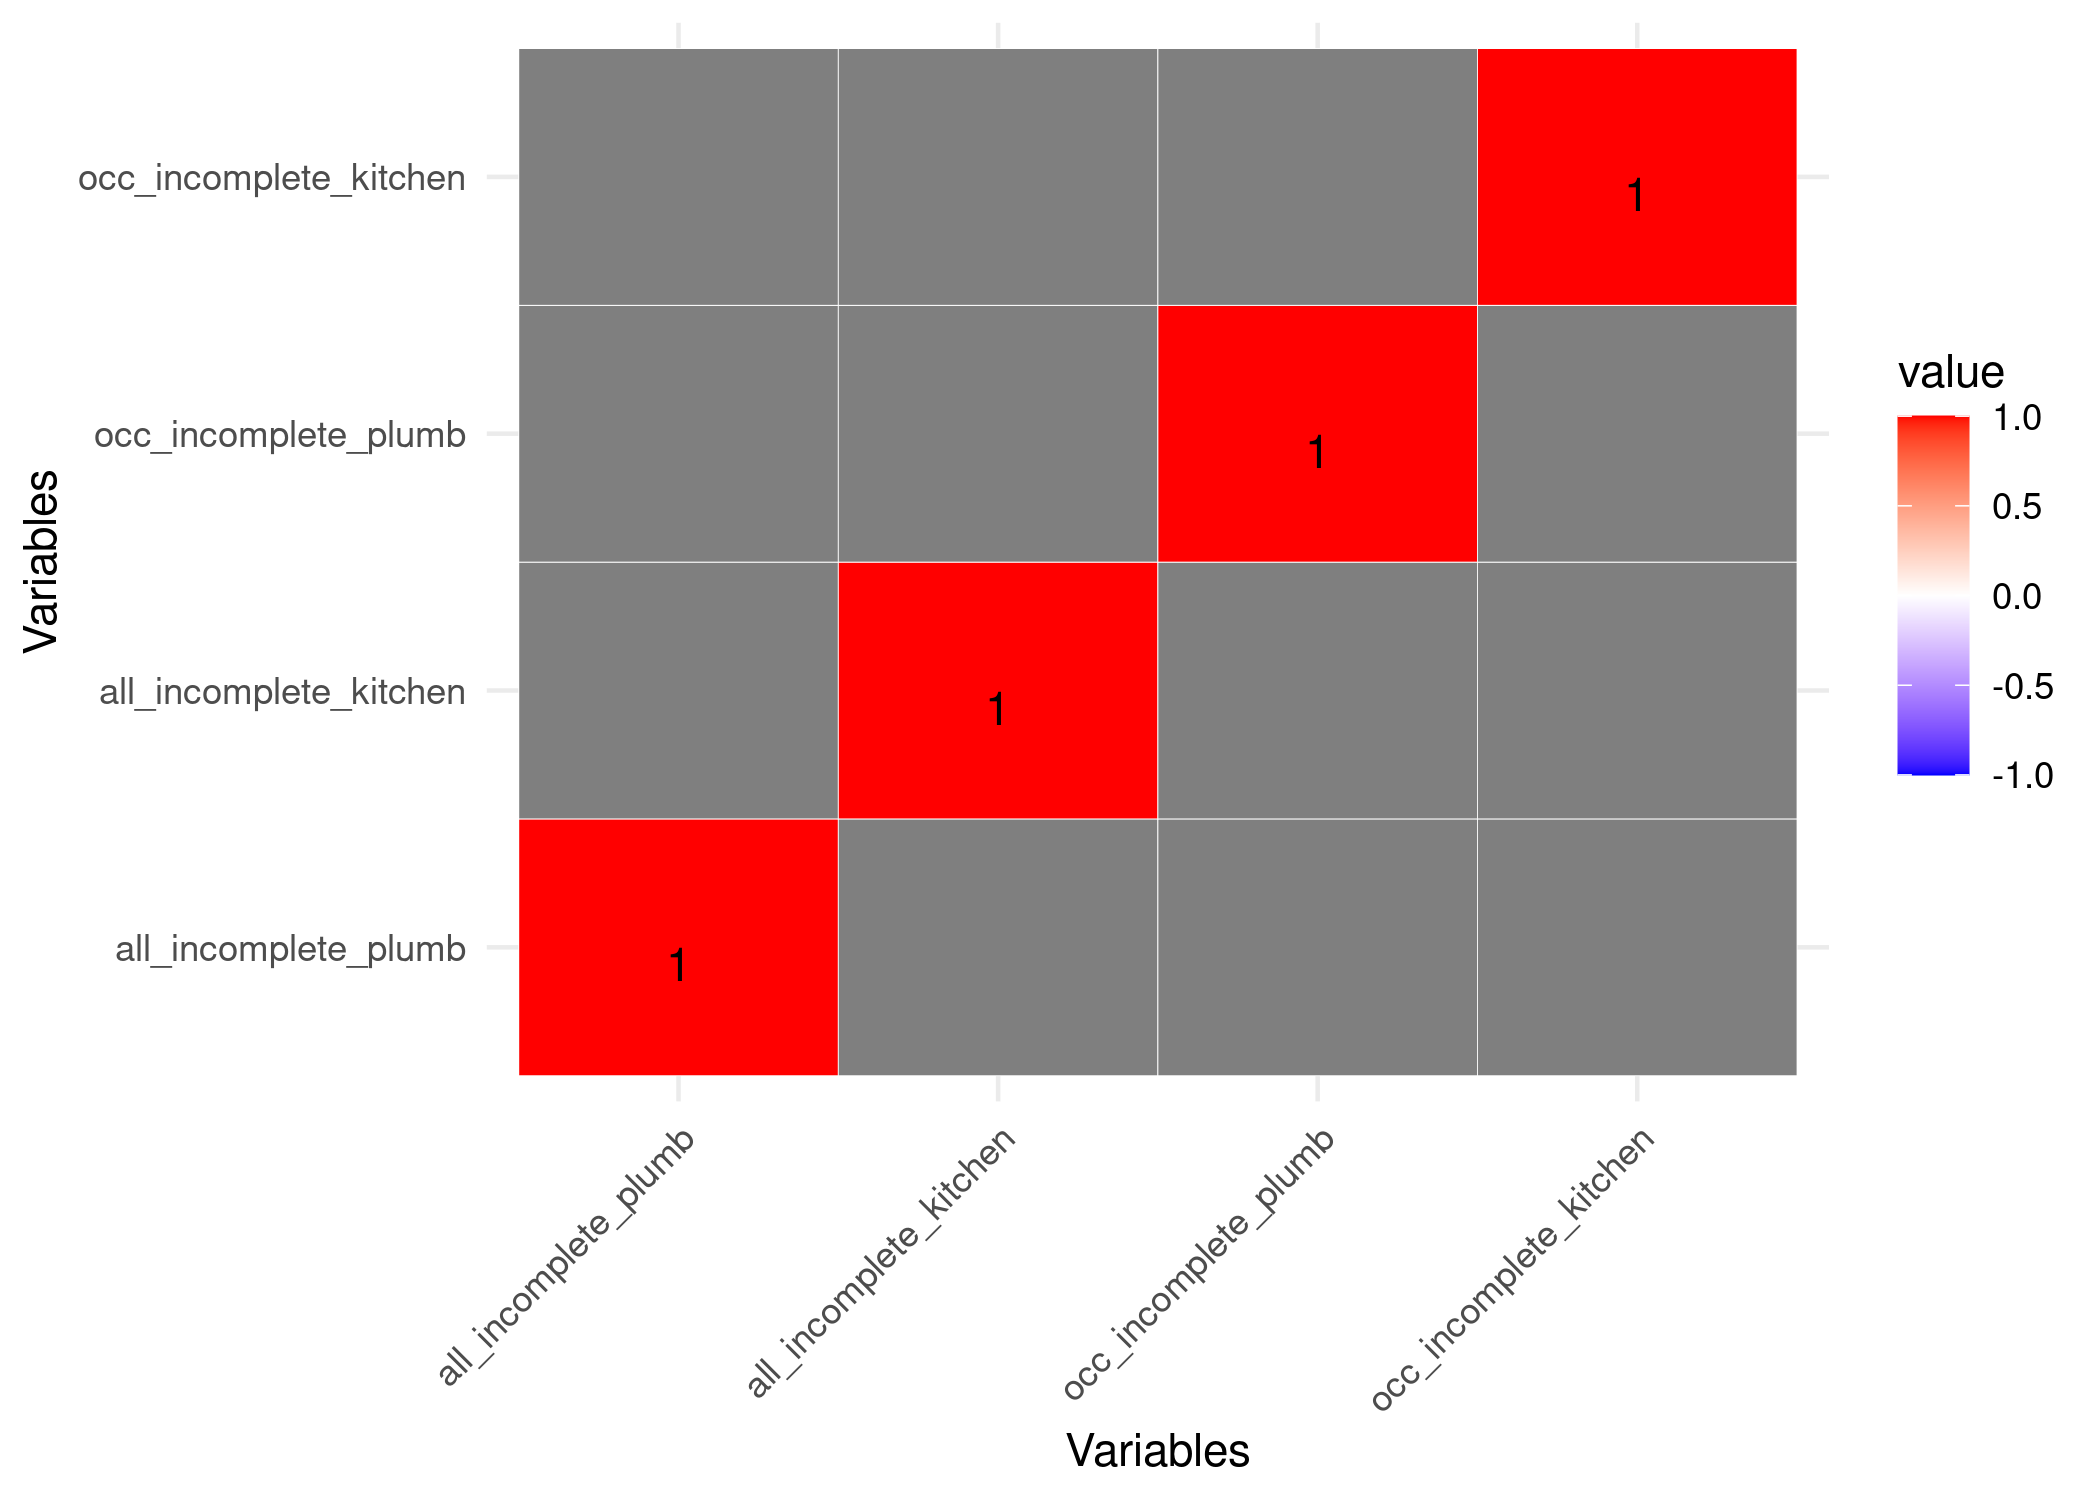
\includegraphics[width=1\textwidth, height=12cm]{plots/correlations/qual_prob_corr.png}
     \caption{Housing Quality Correlation Plot}
 \end{figure}


% okay so this was working but then all the correlations started being NA so i'm not really sure what to do about that. Hopefully future Steve finds this message helpful. it is January 26th and i'm high af 

 \endinput